\subsection{Products and fiber products}

PROPOSITION 2. --- Let B and B' be topological spaces, let (E, p) be a B-space and let (E', p') be a B'-space. Suppose that E and E' are locally trivial fibered spaces (resp. coverings). Then the space E × E', equipped with the map p × p': E × E' → B × B', is a locally trivial fibered space (resp. a covering) with base B × B'. If E and E' are trivializable, then so is E × E'.

Suppose first that the B-space E and the B'-space E' admit trivializations \(g: E \to B \times F\) and \(g': E' \to B' \times F'\). The composite of the homeomorphism \(g \times g'\) of \(E \times E'\) onto \((B \times F) \times (B' \times F')\) with the canonical homeomorphism of \((B \times F) \times (B' \times F')\) onto \((B \times B') \times (F \times F')\) is a trivialization of the \(B \times B'\)-space \(E \times E'\), with fiber type \(F \times F'\). If F and \(F'\) are discrete spaces, the space \(F \times F'\) is also discrete.

In the general case, for any point \((a, a')\) of \(B \times B'\), there exists a neighborhood U of a in B and a neighborhood \(U'\) of \(a'\) in B' such that the U-space \(E_{U}\) and the \(U'\)-space \(E_{U'}\) are trivializable. It follows from the preceding that the \(B \times B'\)-space \(E \times E'\) is trivializable over \(U \times U'\). It is therefore a locally trivial fibered space with base \(B \times B'\). Its fibers are discrete if E and \(E'\) are coverings, whence the proposition.

Note that, if \((p_{i} \colon \mathrm{E}_{i} \to \mathrm{B}_{i})_{i \in \mathrm{I}}\) is a family of locally trivial fiber spaces, or even of coverings, the product space \(\prod_{i \in I} E_{i}\) endowed with the map \((p_{i})_{i \in I}\) is not necessarily a locally trivial fiber space with base \(\prod_{i \in I} B_{i}\) (I, p. 145, exerc. 3).

COROLLARY 1. --- Let A be a topological space, and let B, B' be A-spaces. Let E and E' be locally trivial fibered spaces (resp. coverings) with bases B and B'; denote their projections by p and p'. Then the \(B \times_{A} B'\)-space \(E \times_{A} E'\) obtained from p × p' by passing to subspaces is a locally trivial fibered space (resp. a covering). It is trivializable if E and E' are.

Since the set \(E \times_{A} E'\) is the inverse image of \(B \times_{A} B'\) by the mapping \(p \times p'\) : \(E \times E' \to B \times B'\) , the corollary follows from Proposition 2 and Remark 1 (I, p. 68).

COROLLARY 2. --- Let

\pandocbounded{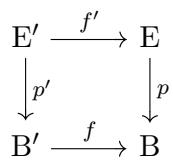
\includegraphics[keepaspectratio]{images/part001_3dd3ce93.jpg}}

a Cartesian square. If (E,p) is a locally trivial B-fibered space (resp. a covering), then (E',p') is a locally trivial fibered space (resp. a covering) with base B', trivializable if (E,p) is.

This follows from Corollary 1, applied with B = A and E' = B'.

COROLLARY 3. --- Let B be a topological space. Let E and E' be locally trivial B-fibered spaces (resp. coverings). Then \(E \times_{B} E'\) is a locally trivial B-fibered space (resp. a covering of B). It is trivializable if E and E' are.

This follows from Corollary 1, applied to the case where A, B, and B' are equal.

PROPOSITION 3. --- Let

\begin{enumerate}
\def\labelenumi{(\arabic{enumi})}
\tightlist
\item
\end{enumerate}

\pandocbounded{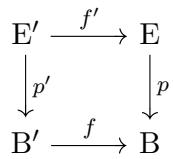
\includegraphics[keepaspectratio]{images/part001_0991252f.jpg}}

a Cartesian square. Suppose that in a neighborhood of every point of B, the map f has a continuous section. Then, if (E', p') is a locally trivial B'-fibered space (resp. a covering), the B-space (E, p) is a locally trivial fibered space (resp. a covering).

We need to prove that every point \(a\) of B has a neighborhood U such that the U-space induced by \((\mathrm{E}, p)\) over U is a locally trivial fibered space (resp. a covering). Take U to be a neighborhood of \(a\) over which there exists a continuous section \(s\) of \(f\). Denote by \(i: \mathrm{U} \to \mathrm{B}\) and \(j: \overline{p}^{-1}(\mathrm{U}) \to \mathrm{E}\) the canonical injections. Since square (1) is Cartesian, there exists a unique continuous map \(s^{\prime}\colon \overline{p}^{1}(\mathrm{U})\to \mathrm{E}^{\prime}\) such that \(f^{\prime}\circ s^{\prime} = j\) and \(p^{\prime}\circ s^{\prime} = s\circ p_{\mathrm{U}}\). The square

\[
\begin{array}{c} \stackrel {{- 1}} {{p}} (\mathrm{U}) \xrightarrow {s ^ {\prime}} \mathrm{E} ^ {\prime} \\ \Biggl \downarrow p _ {\mathrm{U}} \\ \mathrm{U} \xrightarrow {s} \mathrm{B} ^ {\prime} \end{array}\tag{2}
\]

is thus commutative, and its composite with square (1) is the Cartesian square.

\[
\begin{array}{c} \overline {{p}} ^ {1} (\mathrm{U}) \xrightarrow {j} \mathrm{E} \\ \Biggl \downarrow p _ {\mathrm{U}} \\ \mathrm{U} \xrightarrow {i} \mathrm{B}. \end{array}
\]

By proposition 7 of I, p. 15, the square (2) is Cartesian. Corollary 2 allows us to conclude.

Note. --- If in Proposition 3 one weakens the hypothesis on the map f by assuming only that it is universally strict and surjective, and if \(p'\) is a covering, the map p is étale (I, p. 31, prop. 8) and separated (I, p. 27, prop. 4), but E is not necessarily a covering of B. For example, one can find a topological space B and a locally finite closed covering \((\mathrm{A}_{i})_{i\in\mathrm{I}}\) of B, a B-space \((\mathrm{E},p)\) which is not a covering but such that, for every \(i\in I\), the \(A_{i}\)-induced space \(E_{A_{i}}\) is a covering of \(A_{i}\) (I, p. 146, exerc. 5). For a sufficient condition, see, however, Corollary 4 of I, p. 77.

